\documentclass[11pt]{article}

\usepackage[margin=0.72in]{geometry}
\usepackage[T1]{fontenc}
\usepackage[utf8]{inputenc}
\usepackage{lmodern}
\usepackage{microtype}
\usepackage{xcolor}
\usepackage{graphicx}
\usepackage{booktabs}
\usepackage{tabularx}
\usepackage{array}
\usepackage{longtable}
\usepackage{enumitem}
\usepackage{fancyhdr}
\usepackage{titlesec}
\usepackage{tcolorbox}
\usepackage{listings}
\usepackage{tikz}
\usetikzlibrary{arrows.meta,positioning,fit,backgrounds,shapes.geometric,calc}
\usepackage[hidelinks]{hyperref}
\usepackage{url}

\definecolor{KubeBlue}{HTML}{326CE5}
\definecolor{CloudBlue}{HTML}{1261A0}
\definecolor{Ink}{HTML}{17202A}
\definecolor{Slate}{HTML}{566573}
\definecolor{LightBlue}{HTML}{EEF4FF}
\definecolor{LightGray}{HTML}{F4F6F7}
\definecolor{SoftGreen}{HTML}{ECF8F1}
\definecolor{SoftAmber}{HTML}{FFF7E6}
\definecolor{RuleGray}{HTML}{D5D8DC}

\hypersetup{
  colorlinks=true,
  linkcolor=KubeBlue,
  urlcolor=CloudBlue,
  citecolor=KubeBlue,
  pdftitle={Kubernetes and Cloud Architecture Technical Guide},
  pdfauthor={Technical Architecture Handout}
}

\pagestyle{fancy}
\fancyhf{}
\lhead{\textcolor{Slate}{Kubernetes \& Cloud Architecture}}
\rhead{\textcolor{Slate}{Technical Guide}}
\cfoot{\textcolor{Slate}{\thepage}}
\renewcommand{\headrulewidth}{0.3pt}

\titleformat{\section}{\Large\bfseries\color{Ink}}{\thesection}{0.55em}{}
\titleformat{\subsection}{\large\bfseries\color{KubeBlue}}{\thesubsection}{0.55em}{}
\titleformat{\subsubsection}{\normalsize\bfseries\color{Ink}}{\thesubsubsection}{0.55em}{}
\setlist[itemize]{leftmargin=1.35em,itemsep=2pt,topsep=4pt}
\setlist[enumerate]{leftmargin=1.6em,itemsep=2pt,topsep=4pt}
\setlength{\parindent}{0pt}
\setlength{\parskip}{5pt}
\renewcommand{\arraystretch}{1.18}

\newtcolorbox{keyidea}[1][]{
  colback=LightBlue,
  colframe=KubeBlue,
  boxrule=0.7pt,
  arc=2mm,
  left=2mm,right=2mm,top=1.7mm,bottom=1.7mm,
  title=#1,
  fonttitle=\bfseries
}
\newtcolorbox{warningbox}[1][]{
  colback=SoftAmber,
  colframe=orange!70!black,
  boxrule=0.7pt,
  arc=2mm,
  left=2mm,right=2mm,top=1.7mm,bottom=1.7mm,
  title=#1,
  fonttitle=\bfseries
}
\newtcolorbox{practicebox}[1][]{
  colback=SoftGreen,
  colframe=green!45!black,
  boxrule=0.7pt,
  arc=2mm,
  left=2mm,right=2mm,top=1.7mm,bottom=1.7mm,
  title=#1,
  fonttitle=\bfseries
}

\lstdefinestyle{k8syaml}{
  basicstyle=\ttfamily\small,
  backgroundcolor=\color{LightGray},
  frame=single,
  rulecolor=\color{RuleGray},
  breaklines=true,
  showstringspaces=false,
  columns=fullflexible,
  keepspaces=true,
  xleftmargin=0.5em,
  xrightmargin=0.5em
}

\newcommand{\term}[1]{\textbf{\textcolor{KubeBlue}{#1}}}
\newcommand{\code}[1]{\texttt{#1}}
\newcommand{\src}[2]{\href{#2}{#1}}

\begin{document}

\begin{center}
{\Huge\bfseries\color{Ink} Kubernetes \& Cloud Architecture}\\[4pt]
{\Large\color{KubeBlue} Technical Guide and Architecture Handout}\\[10pt]
{\small\color{Slate} Cloud infrastructure, Kubernetes control planes, provider integrations, autoscaling, portability, security, and managed-service responsibility}\\[6pt]
{\small\color{Slate} Source baseline: official Kubernetes, AWS, Google Cloud, and Microsoft documentation; reviewed September 2026}
\end{center}

\vspace{0.4em}
\begin{keyidea}[Core architectural principle]
The cloud provides \textbf{programmable infrastructure}; Kubernetes provides a \textbf{declarative control plane} that schedules, coordinates, and reconciles containerized workloads while integrating with that infrastructure through provider-specific controllers and standardized extension interfaces.
\end{keyidea}

\tableofcontents
\newpage

\section{Executive Summary}

Kubernetes and cloud architecture operate at complementary layers. A cloud platform supplies compute, networking, storage, identity, load balancing, observability, and other managed services. Kubernetes provides an API-driven orchestration system that continuously attempts to make the runtime state of containerized workloads match a declared desired state.

The common phrase ``Kubernetes is the operating system of the cloud'' is a useful metaphor, but it is not technically exact. Kubernetes is better understood as a \term{distributed orchestration and reconciliation platform}. It does not replace the operating systems on worker nodes, the cloud hypervisor, the physical network, or provider control planes.

A production Kubernetes-on-cloud design therefore spans several architectural planes:

\begin{itemize}
  \item \textbf{Cloud infrastructure plane}: virtual machines, networks, block/file storage, load balancers, IAM, DNS, and physical infrastructure.
  \item \textbf{Kubernetes control plane}: API server, scheduler, controller manager, backing state store, admission and policy controls.
  \item \textbf{Cluster data plane}: worker Nodes, kubelet, container runtime, Pod networking, service forwarding, and workload execution.
  \item \textbf{Provider integration plane}: cloud-controller-manager, load-balancer controllers, CSI storage drivers, CNI networking implementations, and node autoscalers.
  \item \textbf{Application plane}: Deployments, StatefulSets, Jobs, Services, ConfigMaps, Secrets, and application-specific controllers.
\end{itemize}

\begin{warningbox}[Important misconception]
Kubernetes improves portability, but it does \textbf{not} eliminate cloud-provider coupling. Kubernetes-native workload objects are portable; IAM, storage classes, managed databases, cloud load-balancer annotations, DNS, observability, messaging, and other provider services can remain cloud-specific.
\end{warningbox}

\section{Layered Architecture}

\begin{center}
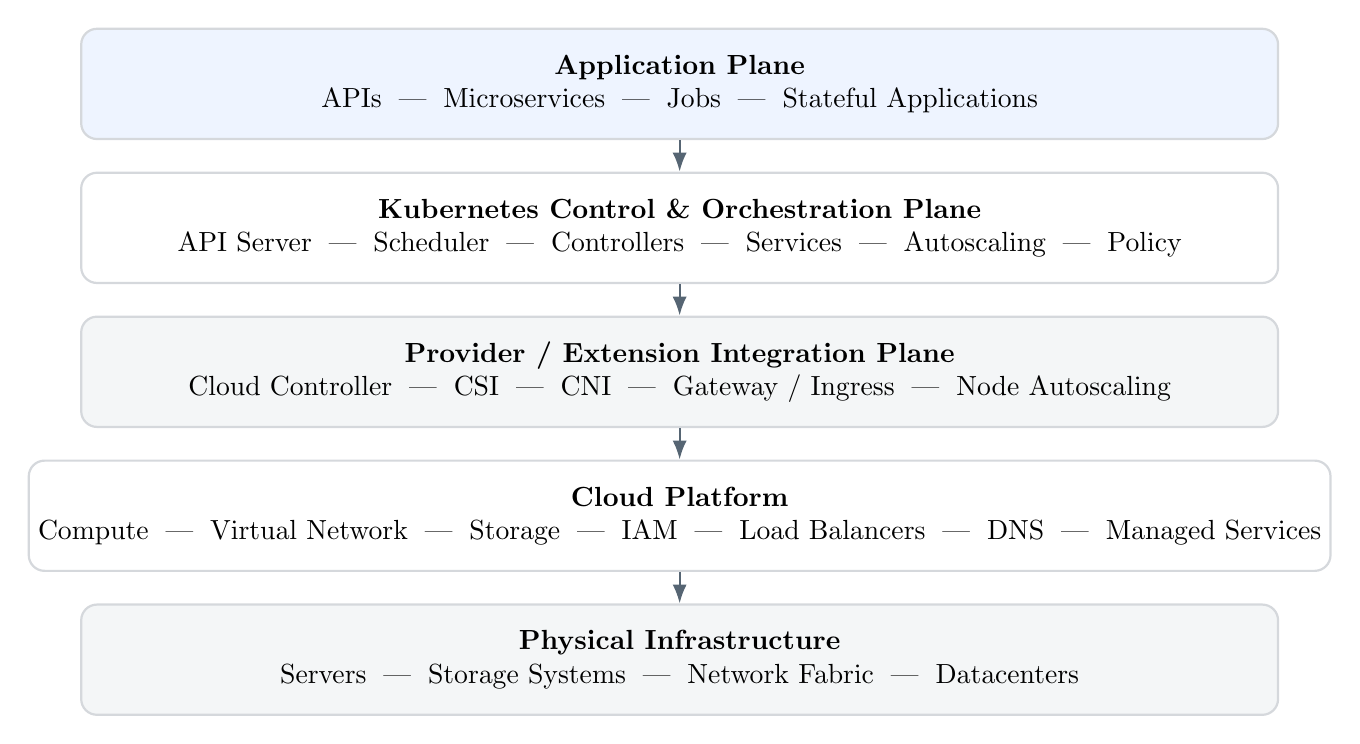
\begin{tikzpicture}[
  node distance=4mm,
  box/.style={draw=RuleGray, rounded corners=2mm, minimum width=15.2cm, minimum height=1.4cm, align=center, thick, fill=white},
  arr/.style={-{Latex[length=2.4mm]}, thick, draw=Slate}
]
\node[box, fill=LightBlue] (apps) {\textbf{Application Plane}\\APIs \;|\; Microservices \;|\; Jobs \;|\; Stateful Applications};
\node[box, below=of apps] (k8s) {\textbf{Kubernetes Control \& Orchestration Plane}\\API Server \;|\; Scheduler \;|\; Controllers \;|\; Services \;|\; Autoscaling \;|\; Policy};
\node[box, below=of k8s, fill=LightGray] (int) {\textbf{Provider / Extension Integration Plane}\\Cloud Controller \;|\; CSI \;|\; CNI \;|\; Gateway / Ingress \;|\; Node Autoscaling};
\node[box, below=of int] (cloud) {\textbf{Cloud Platform}\\Compute \;|\; Virtual Network \;|\; Storage \;|\; IAM \;|\; Load Balancers \;|\; DNS \;|\; Managed Services};
\node[box, below=of cloud, fill=LightGray] (phys) {\textbf{Physical Infrastructure}\\Servers \;|\; Storage Systems \;|\; Network Fabric \;|\; Datacenters};
\draw[arr] (apps) -- (k8s);
\draw[arr] (k8s) -- (int);
\draw[arr] (int) -- (cloud);
\draw[arr] (cloud) -- (phys);
\end{tikzpicture}
\end{center}

\subsection{Cloud responsibility}
The cloud provider exposes programmable resources and APIs. Depending on the service model, those resources may include virtual machines, managed node pools, virtual networks, firewall controls, block storage, load balancers, container registries, identity systems, secrets managers, managed databases, telemetry platforms, and serverless services.

\subsection{Kubernetes responsibility}
Kubernetes supplies a standard API model for declaring and reconciling workload state. The scheduler selects an eligible \term{Node already registered with the cluster}; it does not search arbitrary virtual machines throughout a cloud account. If more capacity is required, a separate node-scaling mechanism may provision infrastructure and join additional Nodes to the cluster.

\section{Control Plane and Data Plane}

A Kubernetes cluster is conventionally divided into a \term{control plane} and a \term{data plane}.

\subsection{Control plane}
The control plane maintains desired cluster state and coordinates reconciliation. Principal components include:

\begin{itemize}
  \item \textbf{kube-apiserver}: the front door for the Kubernetes API and the system's primary coordination interface.
  \item \textbf{kube-scheduler}: assigns unscheduled Pods to suitable Nodes according to resource availability and scheduling constraints.
  \item \textbf{kube-controller-manager}: runs controllers that continuously reconcile Kubernetes objects toward desired state.
  \item \textbf{Cluster state store}: typically \code{etcd} or a provider-managed compatible implementation.
  \item \textbf{Cloud-controller-manager}: hosts cloud-specific controllers when the deployment uses an external cloud-provider integration.
\end{itemize}

\subsection{Data plane}
Worker Nodes execute application workloads. Common Node-level components include:

\begin{itemize}
  \item \textbf{kubelet}: ensures the containers described by Pod specifications are running on the Node.
  \item \textbf{Container runtime}: commonly containerd; executes containers via the Kubernetes Container Runtime Interface ecosystem.
  \item \textbf{Pod networking implementation}: frequently delivered through a CNI-compatible implementation.
  \item \textbf{Service forwarding implementation}: often kube-proxy or equivalent dataplane logic supplied by a networking implementation.
\end{itemize}

\section{Cloud Provider Integration}

\subsection{Cloud Controller Manager}
The \term{cloud-controller-manager (CCM)} separates cloud-specific control logic from cloud-agnostic Kubernetes control-plane logic. Kubernetes documentation describes it as a component that links the cluster to the cloud provider's API and allows cloud providers to evolve their integrations independently of the main Kubernetes codebase.\footnote{Kubernetes, \src{Cloud Controller Manager}{https://kubernetes.io/docs/concepts/architecture/cloud-controller/}.}

Typical CCM responsibilities include Node lifecycle/cloud metadata integration, routes where applicable, and cloud-backed Service functionality. Storage is no longer best described as a generic CCM responsibility; persistent storage is primarily integrated through the Kubernetes storage APIs and CSI ecosystem.

\subsection{External load balancing}
A Kubernetes Service provides a stable network abstraction in front of changing Pod backends. For a Service of \code{type: LoadBalancer}, Kubernetes requires an external load-balancing implementation. Kubernetes itself does not provide the external load balancer. A cloud-provider integration or other controller provisions and configures it.\footnote{Kubernetes, \src{Service}{https://kubernetes.io/docs/concepts/services-networking/service/}.}

\begin{center}
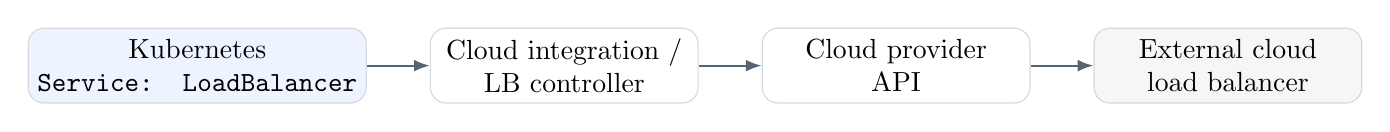
\begin{tikzpicture}[
 n/.style={draw=RuleGray, rounded corners=2mm, align=center, minimum width=3.4cm, minimum height=0.95cm, fill=white},
 a/.style={-{Latex[length=2mm]}, thick, draw=Slate}, node distance=8mm
]
\node[n, fill=LightBlue] (svc) {Kubernetes\\\code{Service: LoadBalancer}};
\node[n, right=of svc] (ctl) {Cloud integration /\\LB controller};
\node[n, right=of ctl] (api) {Cloud provider\\API};
\node[n, right=of api, fill=LightGray] (lb) {External cloud\\load balancer};
\draw[a] (svc) -- (ctl);
\draw[a] (ctl) -- (api);
\draw[a] (api) -- (lb);
\end{tikzpicture}
\end{center}

\begin{lstlisting}[style=k8syaml,caption={Minimal Kubernetes Service requesting an external load balancer}]
apiVersion: v1
kind: Service
metadata:
  name: web
spec:
  selector:
    app: web
  ports:
    - port: 443
      targetPort: 8443
  type: LoadBalancer
\end{lstlisting}

\subsection{Gateway and Ingress}
For HTTP(S) and more advanced north-south traffic control, cloud architectures commonly use Gateway API or Ingress implementations rather than one cloud load balancer per application Service. The Kubernetes networking documentation identifies Gateway API and Ingress as mechanisms for exposing Services beyond the cluster; Gateway implementations may be cloud-specific, bare-metal-oriented, or generic.\footnote{Kubernetes, \src{Services, Load Balancing, and Networking}{https://kubernetes.io/docs/concepts/services-networking/}.}

\section{Persistent Storage and CSI}

Persistent storage is represented through Kubernetes API objects rather than direct application calls to cloud disk APIs.

\begin{center}
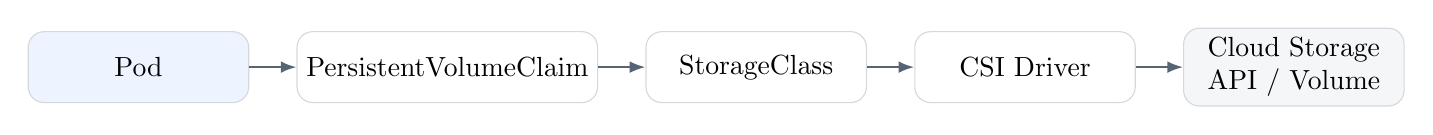
\begin{tikzpicture}[
 n/.style={draw=RuleGray, rounded corners=2mm, align=center, minimum width=2.8cm, minimum height=0.9cm, fill=white},
 a/.style={-{Latex[length=2mm]}, thick, draw=Slate}, node distance=6mm
]
\node[n, fill=LightBlue] (pod) {Pod};
\node[n, right=of pod] (pvc) {PersistentVolumeClaim};
\node[n, right=of pvc] (sc) {StorageClass};
\node[n, right=of sc] (csi) {CSI Driver};
\node[n, right=of csi, fill=LightGray] (disk) {Cloud Storage\\API / Volume};
\draw[a] (pod) -- (pvc);
\draw[a] (pvc) -- (sc);
\draw[a] (sc) -- (csi);
\draw[a] (csi) -- (disk);
\end{tikzpicture}
\end{center}

Kubernetes dynamic provisioning creates storage on demand when users create \term{PersistentVolumeClaim} objects, using \term{StorageClass} definitions to identify the provisioner and its parameters.\footnote{Kubernetes, \src{Dynamic Volume Provisioning}{https://kubernetes.io/docs/concepts/storage/dynamic-provisioning/}.}

In a public-cloud deployment, the provisioner is commonly a CSI driver for a cloud block- or file-storage service. Architectural decisions should explicitly capture:

\begin{itemize}
  \item availability zone and topology constraints;
  \item access mode and volume mode;
  \item encryption and key ownership;
  \item backup, snapshot, restore, and disaster-recovery policy;
  \item storage class defaults, reclaim policy, and expansion behavior;
  \item stateful workload failover semantics.
\end{itemize}

\section{Networking Model}

Kubernetes defines a cluster networking model in which each Pod receives an address and Services provide stable endpoints over changing Pod populations. The implementation is delegated to networking components and cloud integrations.\footnote{Kubernetes, \src{Services, Load Balancing, and Networking}{https://kubernetes.io/docs/concepts/services-networking/}.}

A cloud architecture must therefore reconcile two network domains:

\begin{enumerate}
  \item \textbf{Cloud network domain}: VPC/VNet, subnets, route tables, NAT, security groups or equivalent firewall constructs, private endpoints, peering/transit, and external load balancers.
  \item \textbf{Kubernetes network domain}: Pod CIDRs, Service CIDRs, CNI implementation, NetworkPolicy enforcement, DNS, Gateway/Ingress, and service-to-service traffic.
\end{enumerate}

\begin{practicebox}[Design rule]
Treat IP address planning as an architecture concern, not an installation detail. Pod and Service address ranges, VPC/VNet subnet sizing, multi-cluster routing, hybrid connectivity, and cloud-private-service ranges can create hard scaling limits if planned independently.
\end{practicebox}

\section{Elasticity: Workload Scaling and Node Scaling}

Elasticity is not a single Kubernetes mechanism. It is usually the composition of multiple control loops.

\subsection{Workload autoscaling}
The \term{HorizontalPodAutoscaler (HPA)} adjusts the replica count of a scalable workload such as a Deployment or StatefulSet to match observed resource or custom metrics. Kubernetes documents HPA as a periodically executing control loop.\footnote{Kubernetes, \src{Horizontal Pod Autoscaling}{https://kubernetes.io/docs/concepts/workloads/autoscaling/horizontal-pod-autoscale/}.}

\subsection{Node autoscaling}
If increased replica demand creates Pods that cannot fit on existing Nodes, a \term{Node autoscaler} can add capacity. Kubernetes documentation describes Node autoscalers as systems that provision and consolidate Nodes, often by creating or deleting cloud virtual machines.\footnote{Kubernetes, \src{Node Autoscaling}{https://kubernetes.io/docs/concepts/cluster-administration/node-autoscaling/}.}

\begin{center}
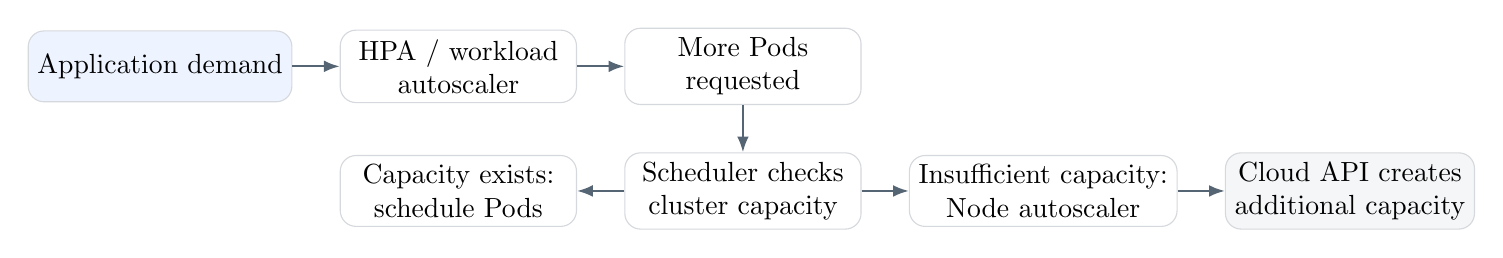
\begin{tikzpicture}[
 n/.style={draw=RuleGray, rounded corners=2mm, align=center, minimum width=3.0cm, minimum height=0.9cm, fill=white},
 a/.style={-{Latex[length=2mm]}, thick, draw=Slate}, node distance=6mm
]
\node[n, fill=LightBlue] (demand) {Application demand};
\node[n, right=of demand] (hpa) {HPA / workload\\autoscaler};
\node[n, right=of hpa] (pods) {More Pods\\requested};
\node[n, below=of pods] (sched) {Scheduler checks\\cluster capacity};
\node[n, left=of sched] (run) {Capacity exists:\\schedule Pods};
\node[n, right=of sched] (na) {Insufficient capacity:\\Node autoscaler};
\node[n, right=of na, fill=LightGray] (cloud) {Cloud API creates\\additional capacity};
\draw[a] (demand) -- (hpa);
\draw[a] (hpa) -- (pods);
\draw[a] (pods) -- (sched);
\draw[a] (sched) -- (run);
\draw[a] (sched) -- (na);
\draw[a] (na) -- (cloud);
\end{tikzpicture}
\end{center}

\subsection{Why the distinction matters}
Adding Pods does not guarantee that compute exists to run them. Conversely, adding Nodes without an appropriate workload scaler does not automatically increase application concurrency. Production architectures should coordinate:

\begin{itemize}
  \item resource requests and limits;
  \item HPA/VPA policy;
  \item node pool or node class definitions;
  \item autoscaler disruption/consolidation policy;
  \item PodDisruptionBudgets and topology spread;
  \item cloud quotas and regional capacity constraints;
  \item startup latency and image-pull time;
  \item cost controls and scale-down behavior.
\end{itemize}

\section{Managed Kubernetes and Shared Responsibility}

There is no universal shared-responsibility table for managed Kubernetes. Responsibility depends on the cloud provider, service, and operating mode.

\begin{table}[ht]
\centering
\small
\begin{tabularx}{\textwidth}{>{\bfseries}p{2.5cm} X X}
\toprule
Service / Mode & Provider-managed emphasis & Customer / platform-team emphasis \\
\midrule
Amazon EKS Standard & AWS manages the Kubernetes control plane. & Workloads, access configuration, cluster add-ons and node/data-plane choices not otherwise delegated. \\
Amazon EKS Auto Mode & AWS extends management into Nodes and core infrastructure capabilities such as compute scaling, networking, load balancing, DNS, and block storage integration. & Workloads, application configuration, governance, and remaining customer-controlled add-ons/policies. \\
GKE Standard & Google manages the control plane and system components; customers retain more worker-node responsibility. & Workloads, cluster configuration, node pools, application resilience, and customer policy. \\
GKE Autopilot & Google manages infrastructure configuration including Nodes, scaling, security defaults, and upgrades. & Workload specifications, application behavior, policy, identity, and data protection choices. \\
AKS & Microsoft provides a managed control plane and manages many system components; some agent-node responsibilities remain shared. & Workloads, user configuration, node maintenance responsibilities where applicable, and application/security policy. \\
\bottomrule
\end{tabularx}
\end{table}

AWS documents that EKS Standard manages the Kubernetes control plane, while EKS Auto Mode extends AWS management into the data plane and associated infrastructure.\footnote{AWS, \src{What is Amazon EKS?}{https://docs.aws.amazon.com/eks/latest/userguide/what-is-eks.html}; \src{Automate cluster infrastructure with EKS Auto Mode}{https://docs.aws.amazon.com/eks/latest/userguide/automode.html}.}

Google documents GKE as a shared-responsibility platform in which Google manages the control plane; in Autopilot, Google also manages worker-node infrastructure and related scaling/maintenance behavior.\footnote{Google Cloud, \src{GKE shared responsibility}{https://cloud.google.com/kubernetes-engine/docs/concepts/shared-responsibility}; \src{GKE Autopilot overview}{https://cloud.google.com/kubernetes-engine/docs/concepts/autopilot-overview}.}

Microsoft documents AKS as providing a managed control plane while identifying several system and agent-node areas as shared responsibility.\footnote{Microsoft Learn, \src{Support policies for Azure Kubernetes Service}{https://learn.microsoft.com/en-us/azure/aks/support-policies}; \src{AKS core concepts}{https://learn.microsoft.com/en-us/azure/aks/core-aks-concepts}.}

\section{Portability and Vendor Coupling}

Kubernetes creates a portable workload API, not a portable cloud in its entirety.

\subsection{Relatively portable layer}
The following Kubernetes abstractions are usually portable with limited changes when applications are designed conservatively:

\begin{itemize}
  \item Deployment, StatefulSet, DaemonSet, Job, and CronJob;
  \item Service, ConfigMap, Secret, and PersistentVolumeClaim;
  \item readiness/liveness/startup probes;
  \item resource requests and limits;
  \item PodDisruptionBudget and topology constraints;
  \item RBAC objects and many admission/policy constructs.
\end{itemize}

\subsection{Common coupling points}
Cloud coupling frequently enters through:

\begin{itemize}
  \item cloud IAM and workload identity;
  \item provider-specific StorageClasses and CSI features;
  \item load-balancer annotations and Gateway implementations;
  \item CNI behavior and IP allocation model;
  \item managed databases, queues, caches, object stores, and event buses;
  \item KMS/secrets systems and certificate services;
  \item cloud-specific observability and security services;
  \item autoscaling APIs and specialized node provisioning;
  \item DNS, private connectivity, and service discovery integrations.
\end{itemize}

\begin{keyidea}[Architectural interpretation]
Kubernetes primarily reduces coupling at the \textbf{workload orchestration interface}. Multi-cloud portability must still be deliberately engineered at the data, identity, network, and managed-service layers.
\end{keyidea}

\section{Security Architecture}

A Kubernetes/cloud security design spans both provider-native and Kubernetes-native controls.

\subsection{Identity and access}
Use cloud IAM for infrastructure/API access and Kubernetes RBAC for cluster-resource authorization. Where available, prefer workload identity mechanisms over distributing long-lived cloud access keys into Pods. Separate human administrative access, CI/CD identities, and workload identities.

\subsection{Network security}
Layer cloud perimeter controls with Kubernetes NetworkPolicy and application-layer ingress/gateway policy. Validate that the selected CNI actually enforces NetworkPolicy; the API can exist even when an implementation does not enforce it.\footnote{Kubernetes, \src{Services, Load Balancing, and Networking}{https://kubernetes.io/docs/concepts/services-networking/}.}

\subsection{Workload hardening}
Architecture baselines should address:

\begin{itemize}
  \item non-root execution and restricted Linux capabilities;
  \item seccomp profiles and OS-level confinement where supported;
  \item read-only filesystems where practical;
  \item signed/provenance-aware container images;
  \item admission policy and namespace guardrails;
  \item secrets lifecycle and external secrets integration;
  \item image and dependency vulnerability management;
  \item runtime and audit telemetry.
\end{itemize}

\subsection{Control-plane security}
Managed services materially reduce control-plane operational burden, but customers still control who can call the Kubernetes API, what those identities may do, which workloads are admitted, and how application/data risks are managed. Google, for example, explicitly documents provider responsibility for hardening and patching the GKE control plane while retaining customer responsibility for workload and configuration choices.\footnote{Google Cloud, \src{GKE shared responsibility}{https://cloud.google.com/kubernetes-engine/docs/concepts/shared-responsibility}.}

\section{Reliability and Failure Domains}

Cloud-native Kubernetes architecture should map Kubernetes scheduling constructs to cloud failure domains.

\begin{itemize}
  \item Spread replicas across Nodes and, where appropriate, zones using topology-spread constraints or anti-affinity.
  \item Use PodDisruptionBudgets to constrain voluntary disruption, but do not treat them as protection against every infrastructure failure.
  \item Ensure storage topology is compatible with failover requirements; a zonal block volume may constrain where a stateful Pod can restart.
  \item Design load balancing, DNS, health checks, and application readiness so traffic follows healthy replicas.
  \item Validate node-autoscaler behavior during zonal shortages and quota exhaustion.
  \item Treat backup/restore and cluster rebuild as separate recovery concerns; Kubernetes manifests alone are not a complete data-protection strategy.
\end{itemize}

\section{Observability and Operations}

Effective operations require visibility across both Kubernetes and cloud layers.

\begin{table}[ht]
\centering
\small
\begin{tabularx}{\textwidth}{>{\bfseries}p{3.1cm} X}
\toprule
Telemetry domain & Typical signals \\
\midrule
Application & request rate, errors, latency, saturation, traces, business KPIs \\
Kubernetes workload & Pod restarts, readiness, OOM kills, throttling, scheduling delay, replica status \\
Kubernetes control plane & API errors/latency, scheduler/controller health, admission failures, etcd/provider state health \\
Node / runtime & CPU, memory, disk pressure, filesystem, kubelet, container runtime, network dataplane \\
Cloud infrastructure & VM health, load balancer health, subnet/IP exhaustion, storage latency, quotas, API throttling \\
Security & audit events, RBAC changes, image findings, policy violations, secrets events, network anomalies \\
\bottomrule
\end{tabularx}
\end{table}

A mature platform correlates these signals. For example, an application latency spike may originate in application code, Pod CPU throttling, Node pressure, cloud load-balancer behavior, storage latency, or a constrained autoscaling path.

\section{Architecture Decision Checklist}

Before selecting or standardizing Kubernetes in a cloud architecture, document the following decisions.

\begin{longtable}{>{\bfseries}p{3.2cm} p{11.8cm}}
\toprule
Decision area & Questions to resolve \\
\midrule
\endhead
Cluster model & Managed or self-managed? Standard or provider-automated mode? Regional or zonal? Single-tenant or shared? \\
Compute & General-purpose, memory/CPU optimized, GPU, spot/preemptible? Node pools/classes? Operating-system requirements? \\
Scaling & HPA/VPA? Node autoscaler? Scaling metrics? Maximum/minimum limits? Consolidation/disruption behavior? \\
Networking & Pod/Service CIDRs? CNI? NetworkPolicy? Ingress/Gateway? Private API? Egress path? Hybrid/multi-cluster routing? \\
Storage & CSI drivers? StorageClasses? Zonal/regional semantics? Encryption? Snapshot/backup/restore? Stateful failover? \\
Identity & Human authentication? Kubernetes RBAC? Workload identity? Break-glass access? CI/CD identities? \\
Security & Pod security baseline? Admission policy? Image controls? Secrets strategy? Runtime detection? Audit retention? \\
Reliability & Failure domains? Replica placement? PDBs? Node maintenance? Quotas? DR and restore objectives? \\
Observability & Logs, metrics, traces, audit events? SLOs? Alerting ownership? Cost attribution? \\
Portability & Which APIs are provider-neutral? Which integrations are intentionally provider-specific? Exit/migration strategy? \\
Governance & Namespace model? Resource quotas? Policy-as-code? Approved registries? Version/upgrade policy? \\
Cost & Node utilization? Autoscaling floors/ceilings? Idle environments? Storage/network egress? Chargeback/showback? \\
\bottomrule
\end{longtable}

\section{Reference Deployment Flow}

The following sequence illustrates how a typical cloud-native deployment crosses responsibility boundaries:

\begin{enumerate}
  \item CI builds a container image and publishes it to a registry.
  \item CD or GitOps submits Kubernetes objects to the API server.
  \item Admission and policy controls validate or mutate the request.
  \item Controllers create the required ReplicaSets, Pods, Services, and other resources.
  \item The scheduler selects Nodes for pending Pods.
  \item The kubelet pulls images and starts containers through the runtime.
  \item The CNI configures Pod networking and the Service dataplane exposes stable service identity.
  \item CSI dynamically provisions or attaches persistent storage when requested.
  \item A cloud or Gateway/load-balancer controller configures north-south access.
  \item HPA or another workload autoscaler adjusts replica counts as demand changes.
  \item A node autoscaler provisions or consolidates cloud compute when the cluster requires more or less capacity.
  \item Cloud and Kubernetes telemetry feed operational, security, reliability, and cost-management systems.
\end{enumerate}

\section{Key Takeaways}

\begin{keyidea}[Summary]
\begin{itemize}
  \item Kubernetes is an orchestration and reconciliation platform, not a replacement for the cloud provider or node operating system.
  \item The cloud supplies infrastructure and APIs; Kubernetes supplies declarative workload and cluster abstractions.
  \item Cloud-controller-manager, CSI, CNI, load-balancer/Gateway controllers, and node autoscalers form key integration boundaries.
  \item Workload autoscaling and node autoscaling are separate control loops that must be designed together.
  \item Managed Kubernetes responsibility varies significantly by provider and service mode.
  \item Kubernetes improves workload portability, but provider-specific identity, networking, storage, and managed services remain major coupling points.
  \item Production architecture must integrate security, observability, reliability, cost, and governance across both Kubernetes and cloud layers.
\end{itemize}
\end{keyidea}

\section*{Official Documentation References}
\addcontentsline{toc}{section}{Official Documentation References}
\begin{enumerate}[leftmargin=1.6em]
  \item Kubernetes. \href{https://kubernetes.io/docs/concepts/architecture/cloud-controller/}{Cloud Controller Manager}.
  \item Kubernetes. \href{https://kubernetes.io/docs/concepts/services-networking/}{Services, Load Balancing, and Networking}.
  \item Kubernetes. \href{https://kubernetes.io/docs/concepts/services-networking/service/}{Service}.
  \item Kubernetes. \href{https://kubernetes.io/docs/concepts/storage/dynamic-provisioning/}{Dynamic Volume Provisioning}.
  \item Kubernetes. \href{https://kubernetes.io/docs/concepts/workloads/autoscaling/}{Autoscaling Workloads}.
  \item Kubernetes. \href{https://kubernetes.io/docs/concepts/workloads/autoscaling/horizontal-pod-autoscale/}{Horizontal Pod Autoscaling}.
  \item Kubernetes. \href{https://kubernetes.io/docs/concepts/cluster-administration/node-autoscaling/}{Node Autoscaling}.
  \item Amazon Web Services. \href{https://docs.aws.amazon.com/eks/latest/userguide/what-is-eks.html}{What is Amazon EKS?}.
  \item Amazon Web Services. \href{https://docs.aws.amazon.com/eks/latest/userguide/automode.html}{Automate cluster infrastructure with EKS Auto Mode}.
  \item Google Cloud. \href{https://cloud.google.com/kubernetes-engine/docs/concepts/shared-responsibility}{GKE shared responsibility}.
  \item Google Cloud. \href{https://cloud.google.com/kubernetes-engine/docs/concepts/autopilot-overview}{GKE Autopilot overview}.
  \item Microsoft Learn. \href{https://learn.microsoft.com/en-us/azure/aks/support-policies}{Support policies for Azure Kubernetes Service}.
  \item Microsoft Learn. \href{https://learn.microsoft.com/en-us/azure/aks/core-aks-concepts}{Azure Kubernetes Service core concepts}.
\end{enumerate}

\vfill
\begin{center}
{\small\color{Slate}Designed as a concise architecture reference for cloud architects, platform engineers, SREs, DevSecOps engineers, and Kubernetes practitioners.}
\end{center}

\end{document}
